%
% chrwilf.tex -- slide template
%
% (c) 2021 Prof Dr Andreas Müller, OST Ostschweizer Fachhochschule
%
\bgroup
\setlength{\abovedisplayskip}{5pt}
\setlength{\belowdisplayskip}{5pt}
\def\kante#1#2{
	\draw[shorten >= 0.2cm,shorten <= 0.2cm] (#1) -- (#2);
}
\def\knoten#1#2{
	\uncover<8->{
		\fill[color=#2!30] (#1) circle[radius=0.2];
		\draw[color=#2] (#1) circle[radius=0.2];
	}
	\only<-7>{
		\draw (#1) circle[radius=0.2];
	}
}
\def\R{1.5}
\definecolor{rot}{rgb}{1,0,0}
\definecolor{gruen}{rgb}{0,0.6,0}
\definecolor{blau}{rgb}{0,0,1}
\begin{frame}[t]
\frametitle{Schranke für die chromatische Zahl}
\vspace{-20pt}
\begin{columns}[t,onlytextwidth]
\begin{column}{0.48\textwidth}
\begin{block}{Satz (Wilf)}
$\uncover<2->{\operatorname{chr}(X) \le 1+}\alpha_{\text{max}} \le\uncover<2->{ 1 + }d$
\end{block}
\uncover<3->{%
\begin{block}{Beispiel}
\begin{align*}
\uncover<4->{d&= 4}
&&\uncover<5->{\Rightarrow& \operatorname{chr}(G) &\le 5}\\
\uncover<6->{\alpha_{\text{max}} &= 
2.9565}
&&\uncover<7->{\Rightarrow& \operatorname{chr}(G) &\le 3}\\
\uncover<4->{\overline{d} &= \frac{24}{9}=\rlap{$2.6666$}}
\end{align*}
\vspace{-20pt}
\begin{center}
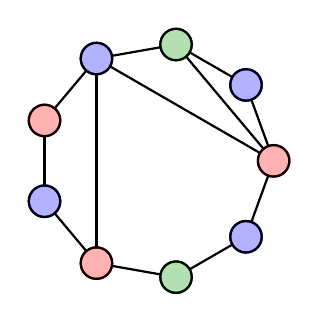
\begin{tikzpicture}[>=latex,thick]

\coordinate (A) at (0:\R);
\coordinate (B) at (40:\R);
\coordinate (C) at (80:\R);
\coordinate (D) at (120:\R);
\coordinate (E) at (160:\R);
\coordinate (F) at (200:\R);
\coordinate (G) at (240:\R);
\coordinate (H) at (280:\R);
\coordinate (I) at (320:\R);

\knoten{A}{rot}
\knoten{B}{blau}
\knoten{C}{gruen}
\knoten{D}{blau}
\knoten{E}{rot}
\knoten{F}{blau}
\knoten{G}{rot}
\knoten{H}{gruen}
\knoten{I}{blau}

\kante{A}{B}
\kante{B}{C}
\kante{C}{D}
\kante{D}{E}
\kante{E}{F}
\kante{F}{G}
\kante{G}{H}
\kante{H}{I}
\kante{I}{A}

\kante{A}{C}
\kante{A}{D}
\kante{D}{G}

\end{tikzpicture}
\end{center}
\end{block}}
\end{column}
\begin{column}{0.52\textwidth}
\uncover<9->{%
\begin{proof}[Beweis]
Induktion nach der Grösse $n$ des Graphen.
\begin{itemize}
\item<10->
Entferne $v\in X$ mit minimalem Grad: $X'=X\setminus \{v\}$
\item<11->
Induktionsannahme:
\[
\operatorname{chr}(X')
\le
1+
\alpha_{\text{max}}' 
\]
\item<12->
$X'$ kann mit höhcstens $1+\alpha_{\text{max}}'\le 1+\alpha_{\text{max}}$
Farben eingefärbt werden.
\item<13->
Wegen
\(
\deg(v) \le \overline{d} \le \alpha_{\text{max}}
\)
hat $v$ höchstens $\alpha_{\text{max}}$ Nachbarn, um $v$ zu färben,
braucht man also höchstens $1+\alpha_{\text{max}}$ Farben.
\end{itemize}
\end{proof}}
\end{column}
\end{columns}
\end{frame}
\egroup
